\documentclass[margin,line]{resume}

\definecolor{sidebarcolor}{RGB}{80, 35, 50}

\usepackage[utf8]{inputenc}
\usepackage[english,russian]{babel}
\usepackage[T1]{fontenc}
\usepackage{fontawesome}

\begin{document}

{\vspace*{-13mm}\sc \large Гришин Антон — Backend разработчик} \\
\begin{resume}
  \begin{minipage}[t]{0.55\textwidth}
    \section{\mysidestyle Персональная\\Информация}
    Москва, Россия \\
    \faHome  \space
    \href{https://alchemmist.xyz}{\texttt{alchemmist.xyz}} \\
    \faGithub  \space
    \href{https://github.com/alchemmist/}{\texttt{alchemmist}} \\
    \faLinkedin \space
    \href{https://www.linkedin.com/in/alchemmist/}{\texttt{alchemmist}}
    \\
    \faPaperPlane \space \href{https://t.me/alchemmist}{\texttt{@alchemmist}} \\
    \faPhone \space
    \href{tel:+1234567890}{\color{blue}\texttt{+7(915)067-2638}}  \\
    \faEnvelope \space
    \href{mailto:anton.ingrish@gmail.com}{\color{blue}\texttt{anton.ingrish@gmail.com}}
  \end{minipage}

  \begin{minipage}[H]{0.18\textwidth}
    % 10.87 1.38
    \begin{textblock}{7}(10.87, 1.38)
      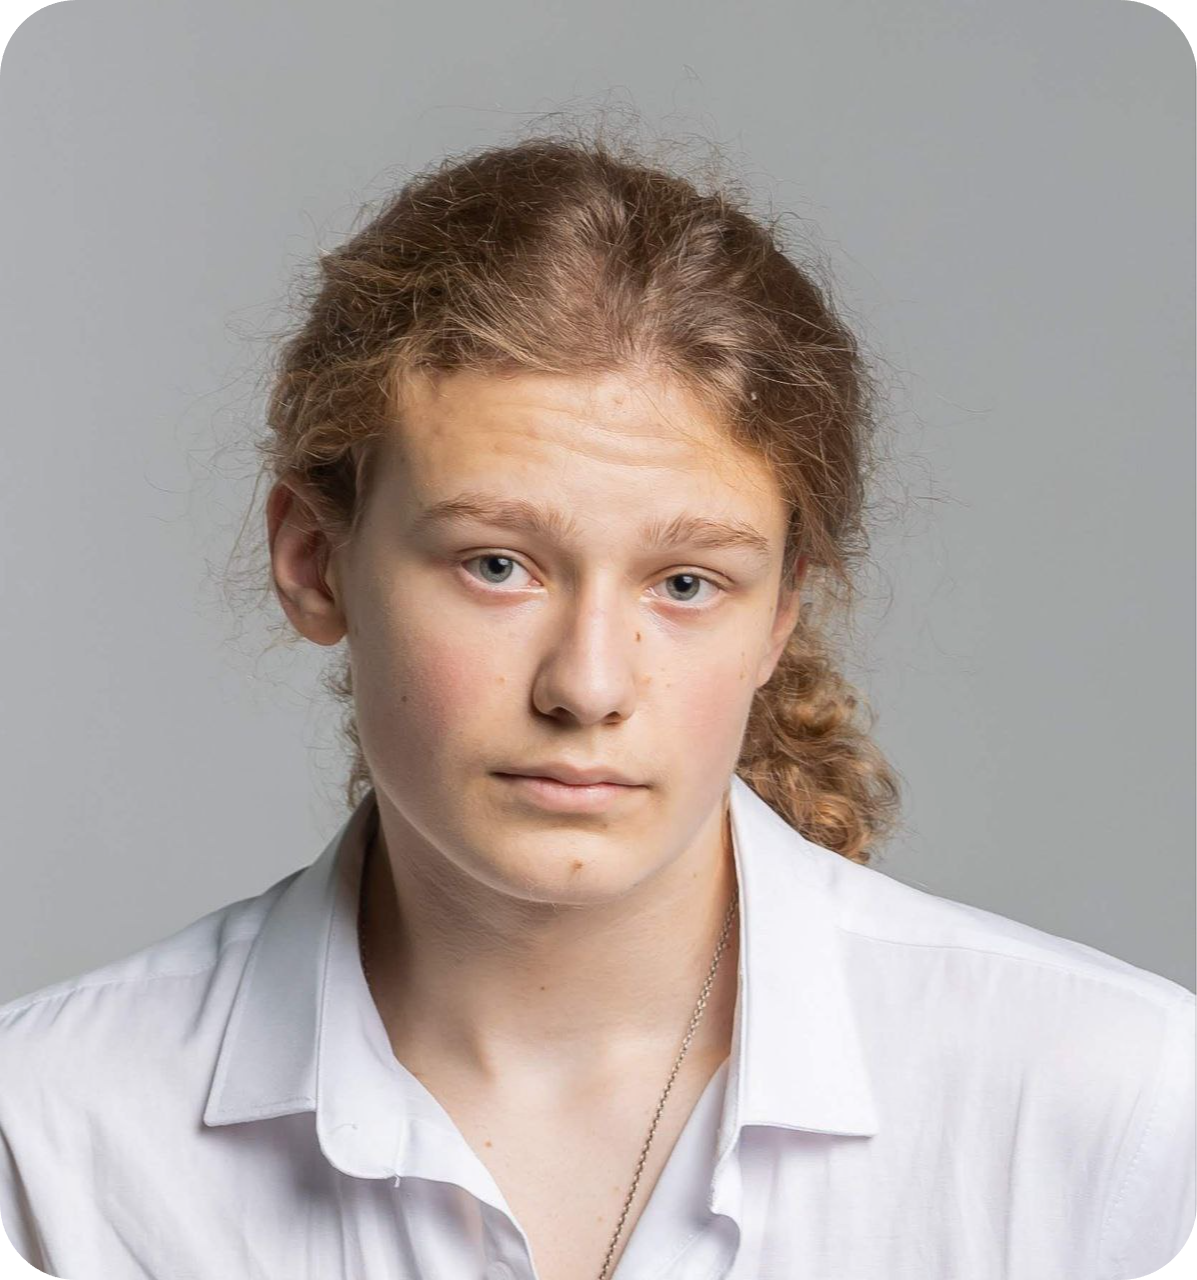
\includegraphics[width=0.270\textwidth]{../images/avatar.png}
    \end{textblock}
  \end{minipage}

  \vspace{-7mm}
  \section{\mysidestyle Обо мне}
  Я студент, начинающий разработчик. Программирую 4 года, за
  это время участвовал в разработке 44 репозиториев, отправил 921
  коммит и написал 176729 строчек кода.
  \href{https://www.avito.ru/moskva/predlozheniya_uslug/prepodavatel_programmirovaniya_na_python_2556461612}{Преподаю}
  Python, обучил $> 30$ учеников. Сооснователь и
  разработчик в \href{https://ballkit.ru/}{Баллкит}. В прошлом профессиональный
  \href{https://alchemmist.github.io/CV/attachments/sport.pdf}{волейболист}.

  \section{\mysidestyle Образование}
  \href{https://centraluniversity.ru/}{Центральный Университет} —
  Математика и компьютерные науки, 2028 \textit{(1 курс)}.
  Направление «Разработка». Траектория «Computer Science Research».

  \section{\mysidestyle Достижения}
  Финалист
  (\href{https://alchemmist.github.io/CV/attachments/russian-chemp-final.pdf}{\texttt{1}})
  \href{https://events.fsp-russia.com/championship}{Чемпионата
  России} по спортивному
  программированию, среди 5000 участников. Технический стек:
  \inlinecode{Kafka}, \inlinecode{React},
  \inlinecode{RabbitMQ (FastStream)},
  \inlinecode{FastAPI},
  \inlinecode{OAuth}.
  % TODO: вложить хакатон на github и добавить ссылку

  \href{https://alchemmist.github.io/CV/attachments/scince-for-life-win.pdf}{Победитель}
  научно-практической конференции
  «\href{https://conf.profil.mos.ru/academ}{Наука для
  жизни}» среди 117 проектов с
  \href{https://github.com/smart-cab/}{проектом умного
  дома}. Технический стек: \inlinecode{Redis},
  \inlinecode{Zigbee2MQTT}, \inlinecode{websockets}, \inlinecode{Go},
  \inlinecode{Python}, \inlinecode{Flask}, \inlinecode{React}.

  Участник хакатона \href{https://nuclearhack.mephi.ru/}{Nuclear
  IT Hack} и
  \href{https://alchemmist.github.io/CV/attachments/informatics-olimpic.pdf}{призёр}
  3-й степени, олимпиады МПГУ по информатике: «Прикладная информатика»

  \section{\mysidestyle Опыт}\vspace{0.7mm}
  \begin{description}[leftmargin=0pt, itemindent=*, itemsep=8pt]
    \item[Ballkit:] Программа лояльности для малого бизнеса.
      Разработал бота в Telegram по модели SMB\textit{(Single Message Bot)} на
      \inlinecode{Go} для коробочной системы лояльности
      \href{https://ballkit.ru}{\texttt{ballkit.ru}}.
      Технологии:
      \inlinecode{Go},
      \inlinecode{tgbotapi}, \inlinecode{grpc},
      \inlinecode{gofsm}.

    \item[Заказная разработка:] Парсеры сложных сайтов
      (\href{https://github.com/alchemmist/portu-hack}{1}).  с
      механизмами авторизации
      (\href{https://github.com/alchemmist/portu-hack/blob/develop/parser/parser/searcher/auth.py}{\texttt{1}}),
      разрешения капчи
      (\href{https://github.com/alchemmist/portu-hack/blob/develop/parser/parser/searcher/captcha.py}{\texttt{2}}),
      и ветвящимся обходом форм
      (\href{https://github.com/alchemmist/portu-hack/blob/develop/parser/parser/searcher/snif.py}{\texttt{3}}).
      Написал
      \href{https://github.com/alchemmist/portu-hack/blob/develop/parser/Dockerfile}{Docker
      образ} для контейнеризованного парсинга
      \inlinecode{selenium} из под движка \texttt{Chromium}.
      Настроил
      \href{https://github.com/alchemmist/portu-hack/blob/develop/pre-commit-config.yaml}{\texttt{pre-commit}}
      хуки для линтера
      \inlinecode{ruff} и статического анализатора \inlinecode{pyright}.
      Технологии:
      \inlinecode{Python}, \inlinecode{selenium},
      \inlinecode{psycopg},
      \inlinecode{SQLALchemy},
      \inlinecode{FastAPI}.

      \vspace{-2mm}
    \item[]\vspace{1mm}\hypersetup{urlcolor=gray!90}\large
      \href{https://github.com/alchemmist}{→ больше проектов на
      \underline{GitHub}}
      \vspace{-3mm}
  \end{description}
  \section{\mysidestyle Сертификаты}
  \textbf{Яндекс Лицей}. Окончил курс
  \href{https://lyceum.yandex.ru/}{Лицея
  Академии Яндекса} по «Промышленной Разработке» с
  \href{https://alchemmist.github.io/CV/attachments/yandex-lyceum.pdf}{аттестатом
  с отличием}, защитив финальный проект на 100/100 баллов.

  \section{\mysidestyle Интересы}\vspace{0.7mm}

  {\textbf{Формальная верификация:} Прохожу курс
    \texttt{\href{https://softwarefoundations.cis.upenn.edu}{softwarefoundations}}.
    Прочитал первый том,
    \href{https://github.com/alchemmist/coq-learning}{доказал} 250
  теорем на \inlinecode{Coq}.} \\

  \vspace{-6mm}

  \textbf{Linux:} Использую Arch с композитором Hyprland. Опубликовал
  свои
  \href{https:/github.com/alchemmist/.dotfiles}{\texttt{.dotfiles}}.
  С нуля написал свой Neovim
  \href{https://github.com/alchemmist/.dotfiles/tree/main/nvim}{конфиг}
  и цветовую
  \href{https://github.com/alchemmist/nothing.nvim}{тему}.
  Написал более 20 кастомных
  \href{https://github.com/alchemmist/.dotfiles/tree/main/scripts}{скриптов}.

\end{resume}

\begin{minipage}[H]{9.18\textwidth}
  \begin{textblock}{7}(-0.65, 10.5)
    \begingroup
    \hspace{35mm}
    \endgroup
  \end{textblock}

\end{minipage}

\clearpage

\end{document}
